\documentclass{ctexart}
\usepackage{minted}
\setminted{formatcom=\xeCJKVerbAddon}
\usepackage{sourcecodepro}
\usepackage{mwe}
\makeatletter
\newlength\savefboxrule
\newlength\savefboxsep
\edef\example@name{\jobname-example.aux}
\newenvironment{hexample}%
{%
\renewcommand{\minted@FVB@VerbatimOut}[1]{%
  \@bsphack
  \begingroup
    \FV@DefineWhiteSpace
    \def\FV@Space{\space}%
    \FV@DefineTabOut
    \let\FV@ProcessLine\minted@write@detok
    \immediate\openout\FV@OutFile ##1\relax
    \let\FV@FontScanPrep\relax
    \let\@noligs\relax
    \FV@Scan}
\minted@FVB@VerbatimOut{\example@name}}%
{\minted@FVE@VerbatimOut%
  \trivlist\item\relax
  \setlength{\savefboxrule}{\fboxrule}%
  \setlength{\savefboxsep}{\fboxsep}%
  \setlength{\fboxsep}{0.007\textwidth}%
  \setlength{\fboxrule}{0.4pt}%
  \fcolorbox[gray]{0}{0.95}{%
    \begin{minipage}[c]{0.45\textwidth}%
      \setlength{\fboxrule}{\savefboxrule}%
      \setlength{\fboxsep}{\savefboxsep}%
      \small\inputminted[breakanywhere,breaklines=true,numbers=left]{latex}{\example@name}%
    \end{minipage}%
  }%
  \hfill%
  \fbox{%
    \begin{minipage}[c]{0.45\textwidth}%
      \setlength{\fboxrule}{\savefboxrule}%
      \setlength{\fboxsep}{\savefboxsep}%
      \setlength{\parskip}{1ex plus 0.4ex minus 0.2ex}%
      \centering
      \normalsize\input{\example@name}%
    \end{minipage}%
  }%
  \endtrivlist
}
\newenvironment{vexample}%
{%
\renewcommand{\minted@FVB@VerbatimOut}[1]{%
  \@bsphack
  \begingroup
    \FV@DefineWhiteSpace
    \def\FV@Space{\space}%
    \FV@DefineTabOut
    \let\FV@ProcessLine\minted@write@detok
    \immediate\openout\FV@OutFile ##1\relax
    \let\FV@FontScanPrep\relax
    \let\@noligs\relax
    \FV@Scan}
\minted@FVB@VerbatimOut{\example@name}}%
{\minted@FVE@VerbatimOut%
  \trivlist\item\relax
  \setlength{\savefboxrule}{\fboxrule}%
  \setlength{\savefboxsep}{\fboxsep}%
  \setlength{\fboxsep}{0.007\textwidth}%
  \setlength{\fboxrule}{0.4pt}%
  \begin{minipage}[c]{\textwidth}
  \fcolorbox[gray]{0}{0.95}{%
    \begin{minipage}[c]{\textwidth-0.03\textwidth-0.8pt}%
      \setlength{\fboxrule}{\savefboxrule}%
      \setlength{\fboxsep}{\savefboxsep}%
      \small\inputminted[breakanywhere,breaklines=true,numbers=left]{latex}{\example@name}%
    \end{minipage}%
  }\\
  \fbox{%
    \begin{minipage}[c]{\textwidth-0.03\textwidth-0.8pt}%
      \setlength{\fboxrule}{\savefboxrule}%
      \setlength{\fboxsep}{\savefboxsep}%
      \setlength{\parskip}{1ex plus 0.4ex minus 0.2ex}%
      \centering
      \normalsize\input{\example@name}%
    \end{minipage}%
  }%
  \end{minipage}
  \endtrivlist
}
\newenvironment{floatexample}%
{%
\renewcommand{\minted@FVB@VerbatimOut}[1]{%
  \@bsphack
  \begingroup
    \FV@DefineWhiteSpace
    \def\FV@Space{\space}%
    \FV@DefineTabOut
    \let\FV@ProcessLine\minted@write@detok
    \immediate\openout\FV@OutFile ##1\relax
    \let\FV@FontScanPrep\relax
    \let\@noligs\relax
    \FV@Scan}
\minted@FVB@VerbatimOut{\example@name}}%
{\minted@FVE@VerbatimOut%
  \trivlist\item\relax
  \setlength{\savefboxrule}{\fboxrule}%
  \setlength{\savefboxsep}{\fboxsep}%
  \setlength{\fboxsep}{0.007\textwidth}%
  \setlength{\fboxrule}{0.4pt}%
  \fcolorbox[gray]{0}{0.95}{%
    \begin{minipage}[c]{\textwidth-0.03\textwidth-0.8pt}%
      \setlength{\fboxrule}{\savefboxrule}%
      \setlength{\fboxsep}{\savefboxsep}%
      \small\inputminted[breakanywhere,breaklines=true,numbers=left]{latex}{\example@name}%
    \end{minipage}%
  }\par
  \input{\example@name}%
  \endtrivlist
}
\makeatother
\setCJKmainfont{方正楷体_GBK}
\setmainfont{方正楷体_GBK}
\usepackage{pgfornament-han}
\usepackage[left=1.2cm,right=1.2cm,top=2cm,bottom=2cm]{geometry}
\usepackage{tikz}
\usetikzlibrary{intersections,calc,arrows.meta,ducks}
\usepackage{eso-pic}
\usepackage{fontawesome}
\pagestyle{empty}
\usepackage{hyperref}
\hypersetup{
  breaklinks,
  unicode,
  linktoc=all,
  bookmarksnumbered=true,
  bookmarksopen=true,
  colorlinks,
  linkcolor=blue,
  citecolor=blue,
  urlcolor=blue,
  plainpages=false,
  linktocpage
}
\usepackage{pdfpages}
\usepackage{enumerate}
\gdef\tikzname{Ti\emph{k}Z}
\gdef\note#1{{\color{purple}\faExclamationTriangle{}:}#1}
\begin{document}
\includepdf{../cover/cover.pdf}
\section*{前言}
首先申明:这并不是\tikzname{}的标准学习文档,而是作者在学习过程中的一些简单记录,如需获取标准学习文档,请命令行执行 {\,}{\color{magenta}texdoc tikz}。由于作者也仅仅是初学者,文档中错误在所难免,还望读者多多指正!本文档主要适用对象为:(1)同作者水平差不多的,并且记不住命令的,方便查阅;(2)初学者,指的是刚学\tikzname{}甚至还没学的朋友,可以做一个简单的入门。如果您在学习过程中遇到了什么问题或是文档中出现的错误,希望您能与我联系。

\vspace*{1cm}
\begin{flushleft}
    \color{blue!50}
    \faWechat:17628192538\\
    \faQq:1123203930\\
    \faEnvelope:1123203930@qq.com
\end{flushleft}

\vspace*{1cm}
\begin{flushright}
 \today  \\
 芒果不盲 
\end{flushright}

\newgeometry{left=3cm,right=3cm,bottom=2cm,top=2cm}
\tableofcontents
\restoregeometry
\newpage
\AddToShipoutPictureBG{
   \begin{tikzpicture}[remember picture,overlay] 
    \node[scale=0.5]at ([yshift=1cm]current page.south){
        \begin{tikzpicture}
            \duck[signpost=\LARGE\thepage]
        \end{tikzpicture}};
   \end{tikzpicture}

    \begin{tikzpicture}[remember picture,overlay]
        % \node[]at ([yshift=1cm]current page.south){\pgfornamenthan[color=blue,scale=0.07]{50}};
        % \node[scale=1.6,text=blue]at ([yshift=1cm]current page.south){\thepage};
        
        \draw[very thick,blue,double] (current page.south west)rectangle(current page.north east);
    \end{tikzpicture}
    \begin{tikzpicture}[remember picture,overlay,x=12,y=12]
        \pgfornamentline[color=blue]{[yshift=10pt,xshift=10pt]current page.south west}{[yshift=10pt,xshift=-10pt]current page.south east}{12}{80}  
        \pgfornamentline[color=blue]{[xshift=10pt,yshift=10pt]current page.south west}{[xshift=10pt,yshift=-10pt]current page.north west}{20}{80}
        \pgfornamentline[color=blue]{[yshift=-10pt,xshift=10pt]current page.north west}{[yshift=-10pt,xshift=-10pt]current page.north east}{12}{80}
        \pgfornamentline[color=blue]{[xshift=-10pt,yshift=-10pt]current page.north east}{[xshift=-10pt,yshift=10pt]current page.south east}{20}{80}
    \end{tikzpicture}
}
\setcounter{page}{1}
\pagenumbering{arabic}
\section{\tikzname{}是什么?}
简单来说,\tikzname{}是\LaTeX{}内部的一个绘图宏包(package),它的功能很强大,我们常说的一句话就是:“不是它不能,而是我们还不会”。学习\tikzname{}需要我们有足够的耐心,要多“折腾”。
\section{如何加载\tikzname{}}
加载\tikzname{}很简单,首先需要在导言区加载\tikzname{\,}\mintinline{tex}{\usepackage{tikz}},开启\tikzname{}有两种方式:

\begin{minted}{tex}
\begin{tikzpicture}[<option>]
 <code>   
\end{tikzpicture}    
\end{minted}
或者:
\begin{minted}{tex}
\tikz{<code>}     
\end{minted}
\note{实际上,前者我们用得比较多。}
\section{绘图基础}
\subsection{直线,箭头}
画直线的语法是:\mintinline{tex}{\draw[option]<code>;}其中option是可选参数,可以设置:颜色,线宽等等,后面我们会逐步介绍到,另外每个完整的绘图语句结束都应该加上西文分号“;”,这与C语言有些类似。
\begin{hexample}
\begin{tikzpicture}
\draw[] (0,0)--(1,1);
\draw[->] (2,0)--(3,1);
\end{tikzpicture}
\end{hexample}
\subsection{圆}
\begin{hexample}

\begin{tikzpicture}
\draw[blue] (0,0)circle[radius=0.5cm];
\draw[line width=2pt,red] (2,0)circle(0.5cm);
\end{tikzpicture}
\end{hexample}
\note{line width 设置线宽}
\subsection{椭圆}
\begin{hexample}
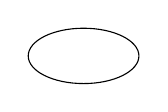
\begin{tikzpicture}
\draw[](0,0)ellipse[x radius=20pt,y radius=10pt];
\end{tikzpicture}
\end{hexample}
\note{这里的 x radius ,y radius 设置长短半轴长。}
\subsection{圆弧}
\begin{hexample}
\begin{tikzpicture}
\draw[] (0,0) arc[start angle=0,end angle=150,radius=1cm];
\draw[yellow] (2.5,0) arc[start angle=0,end angle=180,x radius=1cm,y radius=0.5cm];
\end{tikzpicture}
\end{hexample}
\subsection{矩形}
\begin{hexample}
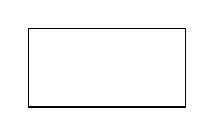
\begin{tikzpicture}
\draw[] (0,0) rectangle (2,1);
\end{tikzpicture}
\end{hexample}
\subsection{网格}
\begin{hexample}

\begin{tikzpicture}
\draw[step=0.5,help lines] (0,0) grid (3,2);    
\end{tikzpicture}
\end{hexample}
\subsection{定义点}
\begin{hexample}
\begin{tikzpicture}
\coordinate[label=left:A] (A) at (0,0);
\coordinate[label=right:B] (B) at (2,2);
\fill[] (A)circle(2pt);
\fill[] (B)circle(2pt);
\draw[] (A)--(B);
\end{tikzpicture}
\end{hexample}
\note{label 用于设置标签,具体用法后续将会介绍。定义点的方法不止于此,后面将会接触到其他方法}
\subsection{坐标}
\tikzname{}中的坐标有两种形式:
\begin{enumerate}
    \item 直角坐标:(x,y),x,y支持任意单位,默认为厘米(cm)。
    \item 极坐标:($\theta$:r),$\theta$表示极角,单位是度;r表示极径。
\end{enumerate}
\begin{hexample}
\tikz{\draw[] (60:1)--(0,0);}
\end{hexample}
\subsection{封闭曲线}
\begin{hexample}
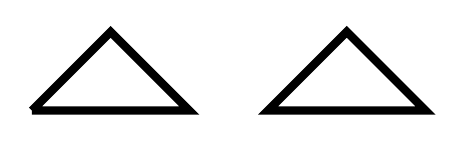
\begin{tikzpicture}
\draw[line width=3pt] (0,0)--(1,1)--(2,0)--(0,0);
\begin{scope}[xshift=3cm]
\draw[line width=3pt] (0,0)--(1,1)--(2,0)--cycle;
\end{scope}
\end{tikzpicture}
\end{hexample}
\subsection{node}
node是在某个坐标放置一些东西,可以是文字,图片,甚至可以插入一段\tikzname{}绘图代码。\\
它的语法为:\mintinline{tex}{\node[<option>](<coordinate name>) at (<coordinate>){<code>};}\\ 
\note{这里的coodinate name是给这个节点(node)命名,方便后面使用,是可以省略的。}
\begin{hexample}
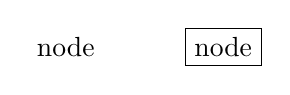
\begin{tikzpicture}
\node[] (a) at (0,0) {node};
\node[draw] at (2,0) {node};
\end{tikzpicture}
\end{hexample}
我们可以观察到,加了一个draw参数,就多了一个外框,实际上节点并不是一个“点”,而(默认)是一个带有大小的矩形。当然也有其它形状咯!既然是矩形,这就不得不谈到它的“锚位”了,它自定义了一些锚位,如center,west,south east等等,我们都可以去引用它们。
\begin{hexample}
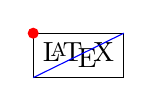
\begin{tikzpicture}
\node[draw] (a) at (0,0) {\LaTeX};
\fill[red] (a.north west) circle (2pt);
\draw[blue] (a.south west)--(a.north east);
\end{tikzpicture}
\end{hexample}
\note{node功能很强大,来日必定再会}
\subsection{填充颜色}\label{3.11}
既然是填充,当然是对封闭路径进行填充了,\tikzname{}会自动加载xcolor宏包,所以我们无需再显示加载了。
\begin{hexample}
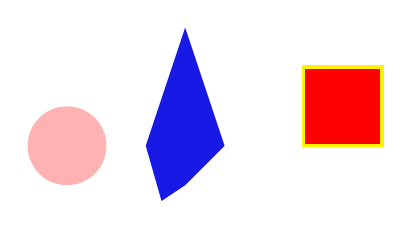
\begin{tikzpicture}
\fill[red!30] (0,0)circle (0.5cm);
\fill[gray!20!blue] (1,0)--(1.5,1.5)--(2,0)--(1.5,-0.5)--(1.2,-0.7)--cycle;
\draw[yellow,fill=red,very thick] (3,0)rectangle ++(1,1);
\end{tikzpicture}
\end{hexample}
\section{进一步探索}
\subsection{美化箭头}
您是否也和我一样,也觉得这个箭头\tikz{\draw[->](0,0)--(1em,1em);}好丑啊,下面我们就来美化它们。我们需要用到\tikzname{}的库了,库之于\tikzname{}的关系如同package之于\LaTeX{}的关系。只需在导言区:\mintinline{tex}{\usetikzlibrary{...}}即可,arrows.meta库提供了很多箭头,以及对箭头的设计,这里我仅仅简单介绍一下,想要深入了解请看\tikzname{}手册。
\begin{hexample}
\begin{tikzpicture}
%\usetikzlibrary{arrows.meta}
\draw[-latex](0,0)--(0,1);
\draw[-Stealth] (1,0)--(1,1);
\draw[-{Triangle[blue]}] (2,0)--(2,1);
\end{tikzpicture}
\end{hexample}
\begin{vexample}
\begin{tikzpicture}[scale=2]
\draw[-{Stealth[length=20pt]}] (0,0)--(0,1); %length:设置箭头长度
\draw[-{Stealth[length=20pt,width=10pt]}] (1,0)--+(0,1); %width:宽度
\draw[-{Stealth[open,color=red]}] (2,0)--+(0,1); %open:空心,相当于fill=none
\draw[-{Stealth[length=10pt,round,fill=blue,red]}] (3,0)--+(0,1); %round:圆角
\draw[-{Stealth[length=10pt,inset=4pt]}] (4,0)--+(0,1);%inset:后角向内移动的距离
\draw[-{Stealth[length=10pt,angle=90:10pt]}] (5,0)--+(0,1); %angle:顶角度数,以及设置箭头的长宽
\draw[-{Stealth[length=10pt,left]}] (6,0)--+(0,1); % left,right:半边箭头,harpoon and harpoon,swap的简写
\draw[-{Stealth[length=10pt,right]}] (7,0)--+(0,1);     
\end{tikzpicture}
\end{vexample}
\note{就简单介绍这些吧,arrows.meta库还有很多箭头样式,可扩展性强,还请阅读\tikzname{}手册。}
\subsection{“+” 和 “++”}
在\tikzname{}中我们用到相对坐标,有时候比起绝对坐标更方便,比如想要做一些修改,如果全用绝对坐标,那将会很糟糕(有可能所有坐标都需要修改)。如果使用相对坐标,工程量就小多了,可能只需要修改极少几个坐标即可做到。但是“+”和“++”有一些区别,前者以第一个点为参考点,后者以前一个点为参考点。
\begin{hexample}

\begin{tikzpicture}
\draw[] (0,0)--+(1,0)--+(1,1)--+(0,1)--cycle;
\begin{scope}[xshift=1.5cm]
\draw[magenta] (0,0)--++(1,0)--++(0,1)--++(-1,0)--cycle;
\end{scope}
\end{tikzpicture}
\end{hexample}
或许你觉得好像区别并不大,别急,我们来画一个六边形。我用“+”,你用“++”。
\begin{hexample}
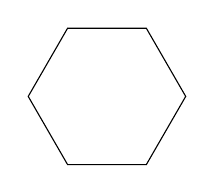
\begin{tikzpicture}
\draw[](0,0)+(0:1)--+(60:1)--+(120:1)--+(180:1)--+(240:1)--+(300:1)--+(360:1)--cycle;
\end{tikzpicture}
\end{hexample}
\note{这里只是简单介绍一下,自行体会吧}
\subsection{shade}
前面\ref{3.11}提到填充颜色,虽然很好,但是它会给整个区域填充同一种颜色,如果我们想要填充一些渐变色呢?
\begin{hexample}

\begin{tikzpicture}
\shade[left color=red,right color=blue] (0,0) rectangle (2,1);
\shade[inner color=white,outer color=gray] (4,0)circle (0.5cm);
\end{tikzpicture}
\end{hexample}
\end{document}